\chapter{ระบบเลขฐาน (Number Bases)}
\label{ch:number-bases}
\zlabel{sec:number-base-intro}

ระบบเลขฐาน คือวิธีเขียนและแทนจำนวนด้วยตัวเลขหลายหลักประกอบกัน โดยค่าของแต่ละตำแหน่งขึ้นอยู่กับฐานของระบบนั้น คอมพิวเตอร์ทำงานด้วยสัญญาณไฟฟ้าสองสถานะ (เปิดและปิด) จึงใช้ระบบเลขฐานสองเป็นภาษาพื้นฐาน การเข้าใจระบบเลขฐานจึงมีความจำเป็นต่อการศึกษาสถาปัตยกรรมคอมพิวเตอร์ การเขียนโปรแกรมระดับต่ำ และการเข้ารหัสข้อมูล~\cite{mano2018digital}

ในชีวิตประจำวัน มนุษย์ใช้ระบบเลขฐานสิบซึ่งมีรากฐานจากการนับนิ้วมือทั้งสิบนิ้ว ในขณะที่อารยธรรมโบราณใช้ระบบฐานที่แตกต่างกัน เช่น ชาวบาบิโลเนียใช้ฐาน 60 ซึ่งยังคงใช้อยู่ในการวัดเวลา (60 วินาที 60 นาที) และการวัดมุม (360 องศา) ส่วนชาวมายาใช้ฐาน 20 แสดงให้เห็นว่าทางเลือกของฐานไม่ได้มีเพียงฐานเดียวที่เป็นธรรมชาติ

ประวัติศาสตร์ของระบบเลขได้พัฒนาผ่านการใช้งานจริงของมนุษยชาติมาอย่างยาวนาน ระบบเลขฐานสิบที่ใช้กันทั่วโลกในปัจจุบันเป็นผลจากการปรับตัวทางวัฒนธรรมและความสะดวกในการใช้งาน ในขณะที่ระบบเลขฐานสองกลายเป็นมาตรฐานในวงการคอมพิวเตอร์เนื่องจากความง่ายในการแทนสถานะทางกายภาพ ไม่ว่าจะเป็นสัญญาณไฟฟ้าสูงและต่ำ หรือสถานะแม่เหล็กบวกและลบ ความสัมพันธ์ระหว่างฐานต่างๆ จึงเป็นเครื่องมือสำคัญในการทำความเข้าใจการทำงานของคอมพิวเตอร์ในทุกระดับ
\label{sec:number-base-intro}

\section{ระบบเลขฐานสิบ (Decimal System)}
\zlabel{sec:decimal-system}
ระบบเลขฐานสิบเป็นระบบเลขตำแหน่ง (Positional Notation) ที่มนุษย์ใช้ในชีวิตประจำวัน โดยใช้เลขโดด 10 ตัว ได้แก่ $0, 1, 2, 3, 4, 5, 6, 7, 8, 9$ ค่าของตัวเลขในแต่ละตำแหน่งจะขึ้นอยู่กับน้ำหนักหรือค่าประจำหลัก ซึ่งคำนวณจากเลขฐาน 10 ยกกำลังด้วยตำแหน่งของหลักนั้น ดังแสดงในรูปที่~\ref{fig:decimal-place-value}

\begin{figure}[H]
    \centering
    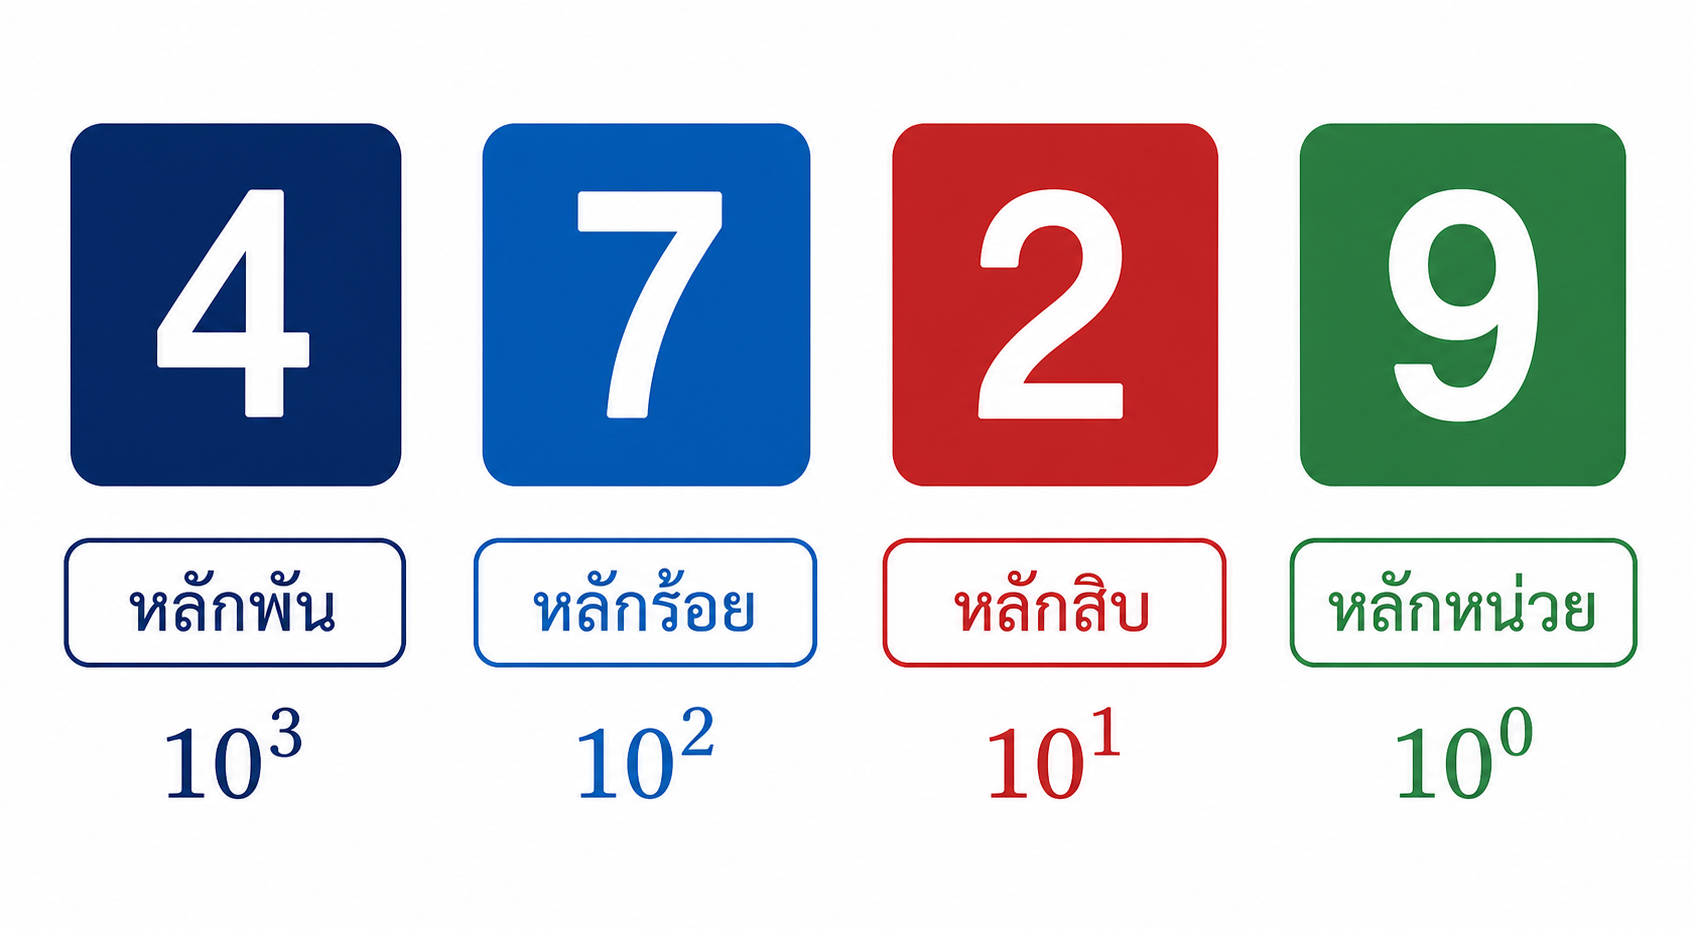
\includegraphics[width=0.62\textwidth]{Figures/png_ready/25-decimal-place-value-manual.png}
    \caption{แผนภาพแสดงค่าประจำหลักของเลขฐานสิบ}
    \label{fig:decimal-place-value}
\end{figure}

ระบบเลขฐานสิบใช้ตัวเลข 10 ตัว และมีฐานเท่ากับ 10 ระบบนี้เป็นระบบที่มนุษย์ใช้มาตลอดประวัติศาสตร์เนื่องจากความสะดวกในการนับด้วยนิ้วมือทั้งสิบนิ้ว การเข้าใจระบบฐานสิบจึงเป็นพื้นฐานสำหรับการศึกษาระบบฐานอื่น

\subsection{ค่าประจำตำแหน่ง}
ในระบบเลขฐานสิบ ค่าของตัวเลขในแต่ละตำแหน่งจะถูกกำหนดโดยผลคูณของตัวเลขหลักนั้นกับ $10^n$ โดย $n$ คือตำแหน่งจากขวาสุดเริ่มนับจากตำแหน่ง 0 สำหรับส่วนจำนวนเต็ม และเริ่มจาก $-1$ ลดลงไปเรื่อยๆ สำหรับส่วนทศนิยม การเข้าใจค่าน้ำหนักประจำหลักนี้เป็นหัวใจสำคัญในการแปลงและทำความเข้าใจระบบเลขฐานอื่นๆ ที่ใช้หลักการเดียวกัน

\begin{thrm}[ค่าประจำตำแหน่งของระบบเลขฐานสิบ]
จำนวนใดๆ ในระบบเลขฐานสิบสามารถเขียนในรูปผลบวกของค่าประจำตำแหน่งได้

$$d_n d_{n-1} \ldots d_1 d_0 . d_{-1} d_{-2} \ldots d_{-m} = \sum_{i=-m}^{n} d_i \times 10^i$$
โดยที่ $d_i$ คือเลขโดดในแต่ละตำแหน่ง และ $10^i$ คือค่าประจำตำแหน่ง
\end{thrm}
\label{thrm:decimal-place-value}

\begin{proof}
การพิสูจน์ค่าประจำตำแหน่งในระบบเลขตำแหน่ง (Positional Notation) พิจารณาเป็นลำดับขั้นตอนดังนี้:
\begin{enumerate}[label=\textbf{\arabic*.}]
    \item \textbf{กำหนดค่าตำแหน่ง:} ให้จำนวนคือ $N = d_n d_{n-1} \ldots d_1 d_0.d_{-1} d_{-2} \ldots d_{-m}$ ในฐาน 10 โดยที่ $d_i$ คือเลขโดดในตำแหน่งที่ $i$
    \item \textbf{คูณน้ำหนักประจำหลัก:} ตัวเลข $d_i$ แต่ละหลักจะมีค่าน้ำหนักเท่ากับกำลังของฐาน 10 นั่นคือ $d_i \times 10^i$
    \item \textbf{รวมผลบวกทุกตำแหน่ง:} นำค่าน้ำหนักทุกหลักตั้งแต่นวนเต็มและส่วนทศนิยมมารวมกัน:
    \[
    N = \sum_{i=-m}^{n} d_i \times 10^i = d_n \times 10^n + d_{n-1} \times 10^{n-1} + \cdots + d_0 \times 10^0 + d_{-1} \times 10^{-1} + \cdots + d_{-m} \times 10^{-m}
    \]
\end{enumerate}
ผลรวมที่ได้สอดคล้องตรงตามนิยามการแทนจำนวนในระบบเลขฐานสิบ
\end{proof}

\begin{ex}[การจำแนกค่าประจำหลักในระบบเลขฐานสิบ]
จงแสดงการกระจายค่าประจำหลักของจำนวนเต็ม $4729$ และจำนวนทศนิยม $53.847$ ในระบบเลขฐานสิบ
\end{ex}
\begin{solution}
สำหรับจำนวนเต็ม $4729$ สามารถกระจายตามค่าประจำหลัก $10^i$ ได้ดังนี้:
\begin{align*}
4729 &= (4\times10^3)+(7\times10^2)+(2\times10^1)+(9\times10^0)\\
     &= 4000+700+20+9
\end{align*}

สำหรับจำนวนทศนิยม $53.847$ สามารถกระจายทั้งส่วนจำนวนเต็มและส่วนทศนิยมได้ดังนี้:
\begin{align*}
53.847 &= (5\times10^1)+(3\times10^0)+(8\times10^{-1})+(4\times10^{-2})+(7\times10^{-3})\\
       &= 50+3+0.8+0.04+0.007
\end{align*}
\solhere
\end{solution}
\label{ex:decimal-place-value}

\section{ระบบเลขฐานสอง (Binary System)}
\zlabel{sec:binary-system}
ระบบเลขฐานสองเป็นระบบเลขพื้นฐานในวิทยาการคอมพิวเตอร์ เนื่องจากวงจรอิเล็กทรอนิกส์และหน่วยความจำของเครื่องคอมพิวเตอร์ทำงานด้วยสัญญาณไฟฟ้าสองสถานะ (เปิดและปิด หรือ สภาวะแรงดันสูงและต่ำ) ระบบนี้ใช้เลขโดดเพียง 2 ตัว คือ $0$ และ $1$ โดยมีค่าประจำหลักเป็นกำลังของฐาน 2 ดังแสดงในรูปที่~\ref{fig:binary-place-value}

\begin{figure}[H]
    \centering
    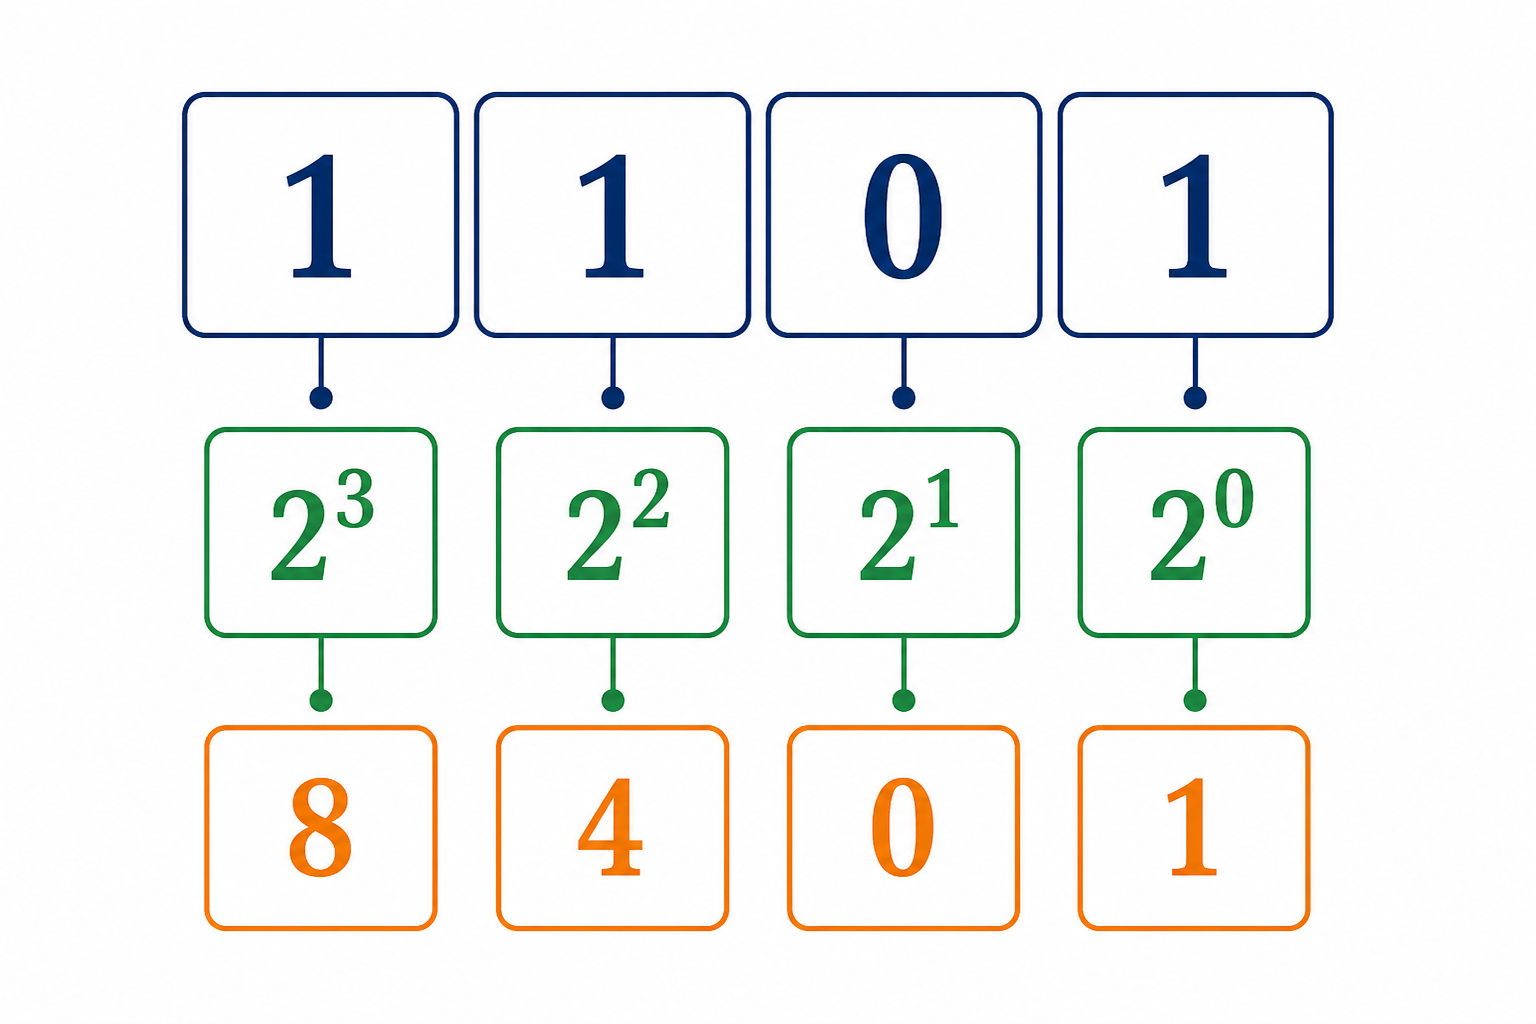
\includegraphics[width=0.62\textwidth]{Figures/png_ready/26-binary-place-value-manual.png}
    \caption{แผนภาพแสดงค่าประจำหลักของเลขฐานสอง}
    \label{fig:binary-place-value}
\end{figure}

รูปที่~\ref{fig:binary-place-value} แสดงบิต $1101$ พร้อมค่าน้ำหนัก $2^3,2^2,2^1,2^0$ ใต้แต่ละตำแหน่ง บิตสามตำแหน่งที่เป็น 1 ให้ค่า $1\times8$, $1\times4$ และ $1\times1$ ส่วนบิตตำแหน่ง $2^1$ เป็น 0 จึงให้ค่าเป็นศูนย์ ดังนั้น $(1101)_2=8+4+0+1=13_{10}$
ระบบเลขฐานสองใช้ตัวเลขเพียง 2 ตัว คือ $0$ และ $1$ และมีฐานเท่ากับ 2 คอมพิวเตอร์ใช้ระบบนี้เพราะวงจรอิเล็กทรอนิกส์สามารถแสดงสองสถานะได้ง่าย (เช่น มีไฟ/ไม่มีไฟ, ปิด/เปิด)
\label{sec:binary-system}

\begin{thrm}
จำนวนในระบบเลขฐานสองสามารถเขียนในรูปผลบวกของ $2^i$ ได้

$$(b_n b_{n-1} \ldots b_1 b_0)_2 = \sum_{i=0}^{n} b_i \times 2^i$$
โดยที่ $b_i \in \{0, 1\}$ แทนเลขโดดแต่ละหลักในฐานสอง
\end{thrm}
\label{thrm:binary-expansion}

\begin{rem}
เลขฐานสอง $(1101)_2$ อ่านว่า ``หนึ่งหนึ่งศูนย์หนึ่งฐานสอง'' ไม่ใช่ ``พันหนึ่งร้อยเอ็ด'' เพราะแต่ละหลักมีค่าประจำตำแหน่งเป็น $2^n$ ไม่ใช่ $10^n$
\end{rem}
\label{rem:binary-reading}

\begin{ex}
แปลง $(1101)_2$ เป็นฐานสิบ
\end{ex}
\begin{solution}
\begin{align*}
(1101)_2 &= (1\times2^3)+(1\times2^2)+(0\times2^1)+(1\times2^0)\\
         &= 8+4+0+1\\
         &= 13
\end{align*}
$\therefore (1101)_2 = (13)_{10}$ \solhere
\end{solution}

\begin{ex}
แปลง $(10110)_2$ เป็นฐานสิบ
\end{ex}
\begin{solution}
\begin{align*}
(10110)_2 &= (1\times2^4)+(0\times2^3)+(1\times2^2)+(1\times2^1)+(0\times2^0)\\
          &= 16+0+4+2+0\\
          &= 22
\end{align*}
$\therefore (10110)_2 = (22)_{10}$ \solhere
\end{solution}

\begin{thrm}
ส่วนทศนิยมในฐานสองมีค่าตามสมการ

$$(0.b_1 b_2 \ldots b_m)_2 = \sum_{i=1}^{m} b_i \times 2^{-i}$$
โดยที่ $b_i \in \{0, 1\}$ แทนเลขโดดในส่วนทศนิยมของฐานสอง
\end{thrm}
\label{thrm:binary-fractional}

\begin{ex}
แปลง $(0.101)_2$ เป็นฐานสิบ
\end{ex}
\begin{solution}
\begin{align*}
(0.101)_2 &= (1\times2^{-1})+(0\times2^{-2})+(1\times2^{-3})\\
          &= \tfrac{1}{2}+0+\tfrac{1}{8}\\
          &= \tfrac{5}{8} = 0.625
\end{align*}
$\therefore (0.101)_2 = (0.625)_{10}$ \solhere
\end{solution}

\begin{ex}
แปลง $(10.011)_2$ เป็นฐานสิบ
\end{ex}
\begin{solution}
\begin{align*}
(10.011)_2 &= (1\times2^1)+(0\times2^0)+(0\times2^{-1})+(1\times2^{-2})+(1\times2^{-3})\\
           &= 2+0+0+0.25+0.125\\
           &= 2.375
\end{align*}
$\therefore (10.011)_2 = (2.375)_{10}$ \solhere
\end{solution}

\section{ระบบเลขฐานแปด (Octal System)}
\zlabel{sec:octal-system}
ระบบเลขฐานแปดใช้ตัวเลข 8 ตัว คือ $0, 1, 2, 3, 4, 5, 6, 7$ และมีฐานเท่ากับ 8 ระบบนี้เคยใช้กันแพร่หลายในยุคแรกของคอมพิวเตอร์เนื่องจากการแปลงระหว่างฐานสองและฐานแปดทำได้ง่าย ทุกตัวเลขฐานแปดสามารถแทนด้วยตัวเลขฐานสอง 3 ตัวพอดี เนื่องจาก $2^3 = 8$ ความสัมพันธ์นี้ทำให้ฐานแปดเป็นวิธีที่สะดวกในการแสดงข้อมูลฐานสองให้อ่านง่ายขึ้น
\label{sec:octal-system}

\begin{thrm}
ความสัมพันธ์ระหว่างฐานสองและฐานแปด: กลุ่มตัวเลขฐานสอง 3 ตัว สามารถแทนด้วยตัวเลขฐานแปด 1 ตัว เนื่องจาก $2^3 = 8$
\end{thrm}
\label{thrm:binary-octal-relation}

\begin{ex}
แปลง $(110101)_2$ เป็นฐานแปด
\end{ex}
\begin{solution}
\begin{align*}
(110101)_2 &= \underbrace{110}_{6}\ \underbrace{101}_{5}\\
           &= (65)_8
\end{align*}
$\therefore (110101)_2 = (65)_8$ \solhere
\end{solution}

\begin{ex}
แปลง $(472)_8$ เป็นฐานสิบ
\end{ex}
\begin{solution}
\begin{align*}
(472)_8 &= (4\times8^2)+(7\times8^1)+(2\times8^0)\\
        &= 256+56+2\\
        &= 314
\end{align*}
$\therefore (472)_8 = (314)_{10}$ \solhere
\end{solution}

\begin{rem}
ฐานแปดเคยใช้กันแพร่หลายในยุคแรกของคอมพิวเตอร์เนื่องจากการแปลงระหว่างฐานสองและฐานแปดทำได้ง่าย ปัจจุบันฐานสิบหกมีการใช้มากกว่า
\end{rem}
\label{rem:octal-history}

\section{ระบบเลขฐานสิบหก (Hexadecimal System)}
\zlabel{sec:hexadecimal-system}
ระบบเลขฐานสิบหกเป็นระบบเลขตำแหน่งที่มีฐานเท่ากับ 16 ใช้สัญลักษณ์ 16 ตัว ประกอบด้วยเลขโดด $0$ ถึง $9$ และตัวอักษรภาษาอังกฤษ $A$ ถึง $F$ (โดย $A=10, B=11, C=12, D=13, E=14, F=15$) ระบบนี้เป็นมาตรฐานในทางคอมพิวเตอร์ เนื่องจากเลขฐานสิบหก 1 หลัก สามารถแทนเลขฐานสองได้ 4 บิตพอดี ช่วยให้ผู้เขียนโปรแกรมอ่านและบันทึกรหัสข้อมูลในหน่วยความจำได้อย่างสะดวก ดังแสดงการจัดกลุ่มในรูปที่~\ref{fig:hex-grouping}

\begin{figure}[H]
    \centering
    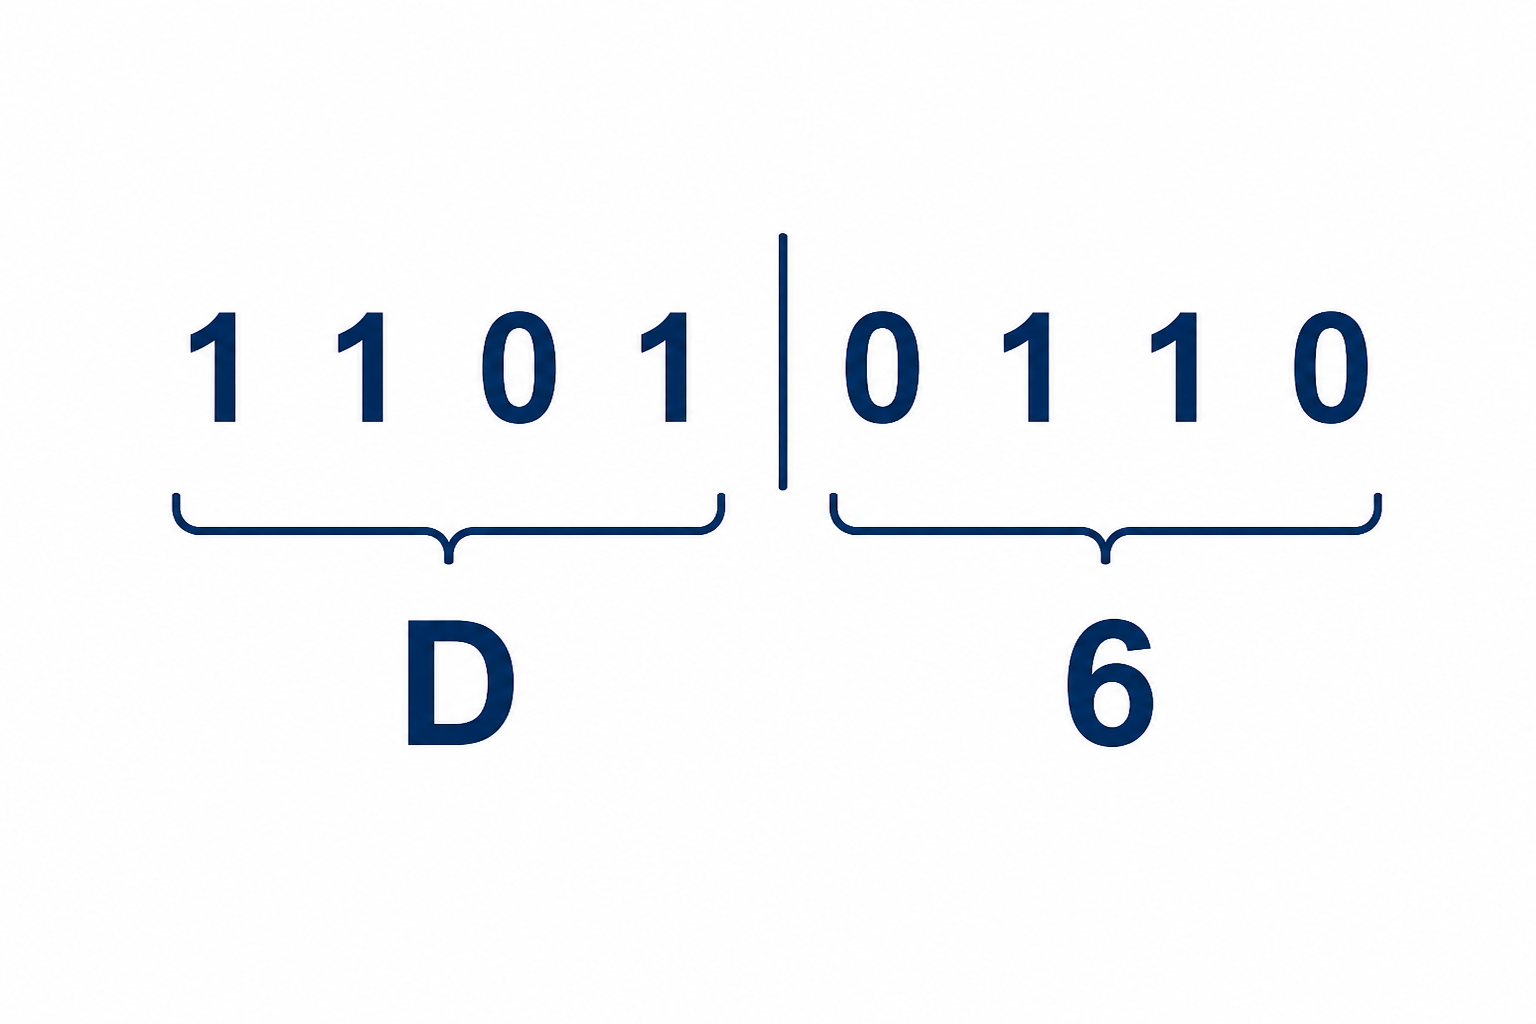
\includegraphics[width=0.62\textwidth]{Figures/png_ready/27-hex-grouping-manual.png}
    \caption{แผนภาพแสดงการจัดกลุ่มเลขฐานสองเป็นเลขฐานสิบหก}
    \label{fig:hex-grouping}
\end{figure}

ระบบเลขฐานสิบหกใช้ตัวเลขและตัวอักษร 16 ตัว คือ $0, 1, 2, 3, 4, 5, 6, 7, 8, 9, A, B, C, D, E, F$ ระบบนี้เป็นมาตรฐานในวงการคอมพิวเตอร์สมัยใหม่เนื่องจากแต่ละตัวอักษรฐานสิบหกแทนได้ด้วยตัวเลขฐานสอง 4 ตัวพอดี เช่นเดียวกับความสัมพันธ์ระหว่างฐานแปดและฐานสอง แต่มีความหนาแน่นของข้อมูลมากกว่าเพราะใช้ทุกตัวในกลุ่ม 4 bits
\label{sec:hexadecimal-system}

\begin{thrm}
ความสัมพันธ์ระหว่างฐานสองและฐานสิบหก: กลุ่มตัวเลขฐานสอง 4 ตัว สามารถแทนด้วยตัวเลขฐานสิบหก 1 ตัว เนื่องจาก $2^4 = 16$
โดยที่แต่ละกลุ่ม 4 bits มีค่าตั้งแต่ $0000_2 = 0$ ถึง $1111_2 = 15 = F_{16}$
\end{thrm}
\label{thrm:binary-hex-relation}

\begin{table}[H]
\centering
\caption{ตารางเปรียบเทียบฐานสิบ ฐานสอง และฐานสิบหก}
\label{tab:binary-hex}
\begin{tabular}{|c|c|c|}
\hline
ฐานสิบ & ฐานสอง (4 หลัก) & ฐานสิบหก \\
\hline
0 & 0000 & 0 \\
1 & 0001 & 1 \\
2 & 0010 & 2 \\
3 & 0011 & 3 \\
4 & 0100 & 4 \\
5 & 0101 & 5 \\
6 & 0110 & 6 \\
7 & 0111 & 7 \\
8 & 1000 & 8 \\
9 & 1001 & 9 \\
10 & 1010 & A \\
11 & 1011 & B \\
12 & 1100 & C \\
13 & 1101 & D \\
14 & 1110 & E \\
15 & 1111 & F \\
\hline
\end{tabular}
\end{table}

\begin{ex}
แปลง $(11010110)_2$ เป็นฐานสิบหก
\end{ex}
\begin{solution}
\begin{align*}
(11010110)_2 &= \underbrace{1101}_{\mathrm{D}}\ \underbrace{0110}_{6}\\
             &= (\mathrm{D}6)_{16}
\end{align*}
$\therefore (11010110)_2 = (\mathrm{D}6)_{16}$ \solhere
\end{solution}

\begin{ex}
แปลง $(3A.F)_{16}$ เป็นฐานสิบ
\end{ex}
\begin{solution}
\begin{align*}
(3A.F)_{16} &= (3\times16^1)+(10\times16^0)+(15\times16^{-1})\\
            &= 48+10+0.9375\\
            &= 58.9375
\end{align*}
$\therefore (3A.F)_{16} = (58.9375)_{10}$ \solhere
\end{solution}

\section{การแปลงฐานทั่วไป}
\zlabel{sec:general-base-conversion}
การแปลงฐานเป็นกระบวนการพื้นฐานที่ใช้ในการสื่อสารระหว่างระบบเลขที่แตกต่างกัน ในทางทฤษฎี การแปลงระหว่างฐานใดๆ สามารถทำได้โดยใช้หลักการของ positional notation ที่สม่ำเสมอ ขั้นตอนการแปลงจะแตกต่างกันขึ้นอยู่กับทิศทางของการแปลงและชนิดของส่วนที่ต้องการแปลง (จำนวนเต็มหรือทศนิยม) การเข้าใจหลักการเบื้องหลังจึงสำคัญกว่าการจำขั้นตอนเพราะทำให้สามารถประยุกต์ใช้กับฐานใดก็ได้
\label{sec:general-base-conversion}

\subsection{การแปลงจากฐานใดๆ เป็นฐานสิบ}
\label{ssec:any-base-to-decimal}
วิธีที่ง่ายที่สุดในการแปลงจากฐานใดๆ เป็นฐานสิบคือการกระจายตามค่าประจำตำแหน่ง

\begin{thrm}
ถ้า $(d_n d_{n-1} \ldots d_1 d_0)_b$ เป็นจำนวนในฐาน $b$ จะมีค่าเท่ากับ

$$(d_n d_{n-1} \ldots d_1 d_0)_b = \sum_{i=0}^{n} d_i \times b^i$$
โดยที่ $d_i$ คือเลขโดดในแต่ละตำแหน่ง และ $b$ คือฐานของระบบเลข
\end{thrm}
\label{thrm:general-base-expansion}

\begin{ex}
แปลง $(2B3)_{16}$ เป็นฐานสิบ และ $(57)_8$ เป็นฐานสิบ
\end{ex}
\begin{solution}
\begin{align*}
(2B3)_{16} &= (2\times16^2)+(11\times16^1)+(3\times16^0)\\
           &= 512+176+3 = 691\\[6pt]
(57)_8     &= (5\times8^1)+(7\times8^0)\\
           &= 40+7 = 47
\end{align*}
$\therefore (2B3)_{16} = (691)_{10}$ และ $(57)_8 = (47)_{10}$ \solhere
\end{solution}

\subsection{การแปลงจากฐานสิบเป็นฐานใดๆ}
\label{ssec:decimal-to-any-base}
ใช้วิธีหารต่อเนื่อง (successive division) โดยหารจำนวนด้วยฐานที่ต้องการแล้วบันทึกเศษ

\begin{thrm}
ขั้นตอนการแปลงจำนวนเต็มจากฐานสิบเป็นฐาน $b$:
\begin{enumerate}
    \item หารจำนวนด้วย $b$ จดเศษไว้
    \item นำผลหารไปหารด้วย $b$ อีก จดเศษ
    \item ทำซ้ำจนกว่าผลหารเป็น 0
    \item เศษที่ได้อ่านจากล่างขึ้นบนคือคำตอบ
\end{enumerate}
\end{thrm}
\label{thrm:decimal-to-any-base-steps}

\begin{ex}
แปลง $45$ ฐานสิบเป็นฐานสอง
\end{ex}
\begin{solution}
\begin{align*}
45 \div 2 &= 22 \quad \text{เศษ } 1\\
22 \div 2 &= 11 \quad \text{เศษ } 0\\
11 \div 2 &= 5  \quad \text{เศษ } 1\\
 5 \div 2 &= 2  \quad \text{เศษ } 1\\
 2 \div 2 &= 1  \quad \text{เศษ } 0\\
 1 \div 2 &= 0  \quad \text{เศษ } 1
\end{align*}
อ่านเศษจากล่างขึ้นบน $\therefore (45)_{10} = (101101)_2$

ตรวจสอบ: $(101101)_2 = 32+8+4+1 = 45$ \checkmark \solhere
\end{solution}

\begin{ex}
แปลง $158$ ฐานสิบเป็นฐานแปด
\end{ex}
\begin{solution}
\begin{align*}
158 \div 8 &= 19 \quad \text{เศษ } 6\\
 19 \div 8 &= 2  \quad \text{เศษ } 3\\
  2 \div 8 &= 0  \quad \text{เศษ } 2
\end{align*}
อ่านเศษจากล่างขึ้นบน $\therefore (158)_{10} = (236)_8$

ตรวจสอบ: $(236)_8 = 128+24+6 = 158$ \checkmark \solhere
\end{solution}

\begin{ex}
แปลง $2543$ ฐานสิบเป็นฐานสิบหก
\end{ex}
\begin{solution}
\begin{align*}
2543 \div 16 &= 158 \quad \text{เศษ } 15\ (\mathrm{F})\\
 158 \div 16 &= 9   \quad \text{เศษ } 14\ (\mathrm{E})\\
   9 \div 16 &= 0   \quad \text{เศษ } 9
\end{align*}
อ่านเศษจากล่างขึ้นบน $\therefore (2543)_{10} = (9\mathrm{EF})_{16}$

ตรวจสอบ: $(9\mathrm{EF})_{16} = 2304+224+15 = 2543$ \checkmark \solhere
\end{solution}

\section{การแปลงจำนวนทศนิยมระหว่างฐาน}
\zlabel{sec:fractional-base-conversion}
การแปลงจำนวนทศนิยมระหว่างฐานมีความซับซ้อนมากกว่าจำนวนเต็มเนื่องจากการคูณต่อเนื่องอาจให้ผลลัพธ์เป็นทศนิยมซ้ำไม่รู้จบในบางฐาน โดยเฉพาะการแปลงทศนิยมฐานสิบเป็นฐานสองนั้น จำนวนที่ดูเหมือนง่ายอย่าง $0.1_{10}$ กลับมีค่าเป็นทศนิยมซ้ำไม่รู้จบในฐานสอง ปรากฏการณ์นี้เป็นที่มาของปัญหา floating-point error ที่พบได้บ่อยในการคำนวณด้วยคอมพิวเตอร์
\label{sec:fractional-base-conversion}

\subsection{การแปลงส่วนทศนิยมจากฐานสิบเป็นฐานอื่น}
\label{ssec:fractional-conversion}
ใช้วิธีคูณต่อเนื่อง (successive multiplication) กับส่วนทศนิยม

\begin{thrm}
ขั้นตอนการแปลงส่วนทศนิยมจากฐานสิบเป็นฐาน $b$:
\begin{enumerate}
    \item คูณส่วนทศนิยมด้วย $b$
    \item บันทึกผลคูณที่เป็นจำนวนเต็ม (0 หรือ 1 สำหรับฐานสอง) เป็นเลขหลักถัดไป
    \item นำส่วนทศนิยมของผลคูณไปคูณต่อ
    \item ทำซ้ำจนกว่าส่วนทศนิยมเป็น 0 หรือได้จำนวนหลักตามต้องการ
\end{enumerate}
\end{thrm}
\label{thrm:fractional-conversion-steps}

\begin{ex}
แปลง $0.625$ ฐานสิบเป็นฐานสอง
\end{ex}
\begin{solution}
\begin{align*}
0.625 \times 2 &= 1.25 \quad \text{หลัก } 1\\
0.25  \times 2 &= 0.5  \quad \text{หลัก } 0\\
0.5   \times 2 &= 1.0  \quad \text{หลัก } 1
\end{align*}
อ่านหลักจากบนลงล่าง $\therefore (0.625)_{10} = (0.101)_2$

ตรวจสอบ: $(0.101)_2 = 0.5+0.125 = 0.625$ \checkmark \solhere
\end{solution}

\begin{ex}
แปลง $0.7$ ฐานสิบเป็นฐานสอง (แสดง 8 หลัก)
\end{ex}
\begin{solution}
\begin{align*}
0.7 \times 2 &= 1.4 \quad \text{หลัก } 1\\
0.4 \times 2 &= 0.8 \quad \text{หลัก } 0\\
0.8 \times 2 &= 1.6 \quad \text{หลัก } 1\\
0.6 \times 2 &= 1.2 \quad \text{หลัก } 1\\
0.2 \times 2 &= 0.4 \quad \text{หลัก } 0\\
0.4 \times 2 &= 0.8 \quad \text{หลัก } 0\\
0.8 \times 2 &= 1.6 \quad \text{หลัก } 1\\
0.6 \times 2 &= 1.2 \quad \text{หลัก } 1
\end{align*}
ส่วนทศนิยม $0.4$ วนซ้ำ ทำให้ได้ทศนิยมซ้ำไม่รู้จบ เมื่อแสดง 8 หลักได้ $(0.7)_{10} \approx (0.10110011)_2$ และค่าที่แท้จริงคือ $(0.7)_{10} = (0.1\overline{0110})_2$ \solhere
\end{solution}

\begin{ex}
แปลง $0.3125$ ฐานสิบเป็นฐานแปด
\end{ex}
\begin{solution}
\begin{align*}
0.3125 \times 8 &= 2.5 \quad \text{หลัก } 2\\
0.5    \times 8 &= 4.0 \quad \text{หลัก } 4
\end{align*}
อ่านหลักจากบนลงล่าง $\therefore (0.3125)_{10} = (0.24)_8$

ตรวจสอบ: $(0.24)_8 = \tfrac{2}{8}+\tfrac{4}{64} = 0.25+0.0625 = 0.3125$ \checkmark \solhere
\end{solution}

\section{การบวกและลบเลขฐานสอง}
\zlabel{sec:binary-add-sub}
การบวกและลบเลขฐานสองเป็นการดำเนินการพื้นฐานที่วงจรคอมพิวเตอร์ใช้ในการคำนวณทุกระดับ หลักการเหมือนกับการบวกลบฐานสิบแต่ใช้ฐาน 2 แทน การเข้าใจการทำงานของ carry และ borrow ในฐานสองจึงเป็นพื้นฐานสำคัญสำหรับการออกแบบ ALU (Arithmetic Logic Unit)
\label{sec:binary-add-sub}

\subsection{การบวกเลขฐานสอง}
การบวกเลขฐานสองมีกฎพื้นฐานดังนี้
\begin{thrm}
การบวกเลขฐานสอง

\begin{enumerate}
    \item $0 + 0 = 0$
    \item $0 + 1 = 1$
    \item $1 + 0 = 1$
    \item $1 + 1 = 10$ (เป็น 0 ทด 1)
    \item $1 + 1 + 1 = 11$ (เป็น 1 ทด 1)
\end{enumerate}
\end{thrm}
\label{thrm:binary-addition-rules}

\begin{ex}
บวก $(1011)_2$ กับ $(1101)_2$:
\end{ex}

\begin{solution}
\[
\begin{array}{r}
1011 \\
+\,1101 \\
\hline
11000
\end{array}
\]
$\therefore (1011)_2 + (1101)_2 = (11000)_2$

ตรวจสอบ: $(1011)_2 = 11_{10}$, $(1101)_2 = 13_{10}$, และ $11+13 = 24 = (11000)_2$ \checkmark \solhere
\end{solution}

\begin{ex}
บวก $(1111)_2$ กับ $(0001)_2$:
\end{ex}

\begin{solution}
\[
\begin{array}{r}
1111 \\
+\,0001 \\
\hline
10000
\end{array}
\]
$\therefore (1111)_2 + (0001)_2 = (10000)_2 = (16)_{10}$ \solhere
\end{solution}

\subsection{การลบเลขฐานสอง}
\label{ssec:binary-subtraction}
การลบเลขฐานสองใช้หลักการขอยืม (Borrowing) ในลักษณะเดียวกับการลบเลขฐานสิบในชีวิตประจำวัน โดยเมื่อตัวตั้งมีค่าน้อยกว่าตัวลบในหลักเดียวกัน จะต้องทำการขอยืมค่าน้ำหนักจากหลักที่อยู่ทางซ้ายมือซึ่งมีค่าเป็น 2 เท่าของหลักปัจจุบัน ในระบบคอมพิวเตอร์ การลบสามารถทำได้ทั้งการลบโดยตรงและการแปลงให้อยู่ในรูปการบวกด้วยส่วนเติมเต็ม (Complement)

\begin{thrm}
การลบเลขฐานสอง

\begin{enumerate}
    \item $0 - 0 = 0$
    \item $1 - 0 = 1$
    \item $1 - 1 = 0$
    \item $0 - 1 = 1$ (ยืม 1 จากหลักซ้าย ทำให้หลักซ้ายลดลง 1)
\end{enumerate}
\end{thrm}
\label{thrm:binary-subtraction-rules}

\begin{ex}
ลบ $(1100)_2$ ด้วย $(0101)_2$:
\end{ex}

\begin{solution}
\[
\begin{array}{r}
1100 \\
-\,0101 \\
\hline
0111
\end{array}
\]
$\therefore (1100)_2 - (0101)_2 = (0111)_2$

ตรวจสอบ: $(1100)_2 = 12_{10}$, $(0101)_2 = 5_{10}$, และ $12-5 = 7 = (0111)_2$ \checkmark \solhere
\end{solution}

\begin{ex}
ลบ $(1000)_2$ ด้วย $(0001)_2$ (แสดงขั้นตอนการยืม)

\end{ex}

\begin{solution}
\[
\begin{array}{r}
1000 \\
-\,0001 \\
\hline
0111
\end{array}
\]
การยืมต่อเนื่อง: หลักขวาสุด $0-1$ ต้องยืมจากหลักที่สี่ผ่านหลักที่สองและสาม ทำให้ $1000_2$ กลายเป็นค่าประจำหลัก $0,1,1,10_2$ ก่อนลบ

$\therefore (1000)_2 - (0001)_2 = (0111)_2$

ตรวจสอบ: $(1000)_2 = 8_{10}$, $(0001)_2 = 1_{10}$, และ $8-1 = 7 = (0111)_2$ \checkmark \solhere
\end{solution}

\section{การคูณและการหารเลขฐานสอง}
\zlabel{sec:binary-mult-div}
การคูณเลขฐานสองมีข้อได้เปรียบที่สำคัญคือผลคูณของแต่ละหลักมีได้เพียง 0 หรือ 1 ทำให้การคูณลดรูปเป็นการ shift และบวก ซึ่งเป็นการดำเนินการที่วงจรดิจิทัลทำได้อย่างมีประสิทธิภาพ หลักการนี้เป็นพื้นฐานของ multiplier ในหน่วยประมวลผลกลาง
\label{sec:binary-mult-div}

\subsection{การคูณเลขฐานสอง}
การคูณเลขฐานสองมีโครงสร้างที่ง่ายและเป็นระเบียบเนื่องจากตัวคูณในแต่ละตำแหน่งมีเพียงสัญลักษณ์ 0 หรือ 1 เท่านั้น เมื่อตัวคูณเป็น 0 ผลคูณย่อยจะเป็น 0 ทั้งหมด และเมื่อตัวคูณเป็น 1 ผลคูณย่อยจะเท่ากับตัวตั้งเดิม กระบวนการคูณในคอมพิวเตอร์จึงลดรูปเหลือเพียงการเลื่อนตำแหน่งบิต (Bit Shift) และการบวกสะสมผลลัพธ์ย่อยเข้าด้วยกัน

\begin{thrm}
การคูณเลขฐานสอง

\begin{enumerate}
    \item $0 \times 0 = 0$
    \item $0 \times 1 = 0$
    \item $1 \times 0 = 0$
    \item $1 \times 1 = 1$
\end{enumerate}
\end{thrm}
\label{thrm:binary-multiplication-rules}

\begin{ex}
คูณ $(1011)_2$ ด้วย $(1101)_2$:
\end{ex}

\begin{solution}
\[
\begin{array}{r}
1011 \\
\times\,1101 \\
\hline
1011 \\
0000\phantom{0} \\
1011\phantom{00} \\
1011\phantom{000} \\
\hline
10001111
\end{array}
\]
$\therefore (1011)_2 \times (1101)_2 = (10001111)_2$

ตรวจสอบ: $(1011)_2 = 11_{10}$, $(1101)_2 = 13_{10}$, และ $11\times13 = 143 = (10001111)_2$ \checkmark \solhere
\end{solution}

\begin{rem}
การคูณเลขฐานสองในคอมพิวเตอร์ใช้วิธี shift-and-add ซึ่งประสิทธิภาพกว่าการคูณแบบธรรมดามาก
\end{rem}
\label{rem:shift-add}

\section{การแทนจำนวนเต็มลบในฐานสอง}
\zlabel{sec:negative-binary}
ในคอมพิวเตอร์ จำนวนเต็มลบต้องมีการแทนที่พิเศษ เนื่องจากไม่มีเครื่องหมายลบในฐานสอง มี 3 วิธีหลักที่ใช้กัน ได้แก่ Signed Magnitude, 1's Complement และ 2's Complement แต่ละวิธีมีข้อดีข้อเสียแตกต่างกัน และมีผลต่อช่วงของจำนวนที่สามารถแทนได้รวมถึงวิธีการบวกลบในระบบ การเข้าใจความแตกต่างของแต่ละวิธีจึงมีความสำคัญต่อการเขียนโปรแกรมระดับต่ำและการออกแบบระบบดิจิทัล
\label{sec:signed-number-representation}

\subsection{Signed Magnitude (Sign-Magnitude)}
\label{ssec:sign-magnitude}
ใช้หลักซ้ายสุดเป็น bit สำหรับเครื่องหมาย (0 = บวก, 1 = ลบ) และหลักที่เหลือเป็นค่าสัมบูรณ์

\begin{thrm}
ในระบบ signed magnitude ขนาด $n$ bits:
\begin{enumerate}
    \item bit ซ้ายสุด = เครื่องหมาย (0 บวก, 1 ลบ)
    \item bits ที่เหลือ = ค่าสัมบูรณ์
    \item ช่วง $-(2^{n-1}-1)$ ถึง $+(2^{n-1}-1)$
    \item มี 0 สองแบบ คือ $+0$ และ $-0$
\end{enumerate}
\end{thrm}
\label{thrm:sign-magnitude}

\begin{ex}
ในระบบ signed magnitude 8 bits: $+45$ และ $-45$ แทนด้วย binary อย่างไร
\end{ex}
\begin{solution}
\begin{align*}
45  &= (0101101)_2 \quad (\text{ส่วนขนาด 7 บิต})\\
+45 &= (\underline{0}\,0101101)_2 = (00101101)_2\\
-45 &= (\underline{1}\,0101101)_2 = (10101101)_2
\end{align*}
โดยบิตซ้ายสุดที่ขีดเส้นใต้คือบิตเครื่องหมาย \solhere
\end{solution}

\begin{rem}
วิธี signed magnitude ไม่ค่อยใช้ในปัจจุบันเพราะมี 0 สองแบบและวงจรลำบาก
\end{rem}
\label{rem:sign-magnitude-rarely-used}

\subsection{1's Complement}
\label{ssec:ones-complement}
การแทนจำนวนลบโดยการกลับ bit ทุก bit ของจำนวนบวก

\begin{thrm}
ในระบบ 1's complement ขนาด $n$ bits:
\begin{enumerate}
    \item ค่าบวก เหมือน unsigned
    \item ค่าลบ คือ กลับ bit ทุก bit ของค่าบวก
    \item ช่วง $-(2^{n-1}-1)$ ถึง $+(2^{n-1}-1)$
    \item ยังมี 0 สองแบบ คือ $+0 = 00000000$, $-0 = 11111111$
\end{enumerate}
\end{thrm}
\label{thrm:ones-complement}

\begin{prop}
ในระบบ 1's complement $n$ bits สำหรับจำนวนเต็ม $x$ ใดๆ ที่ $0 \leq x < 2^{n-1}$ จะได้ว่า $x + \overline{x} = 2^n - 1$ เมื่อ $\overline{x}$ คือ bitwise complement ของ $x$
\end{prop}

\begin{ex}
ในระบบ 1's complement 8 bits:
\end{ex}
\begin{solution}
\begin{align*}
+45 &= (00101101)_2\\
-45 &= (11010010)_2 \quad (\text{กลับบิตทุกบิต})
\end{align*}
การบวกใน 1's complement ต้องมี end-around carry
\[ (00101101)_2 + (11010010)_2 = (11111111)_2 = -0 \]
\end{solution}

\subsection{2's Complement}
\begin{figure}[H]
    \centering
    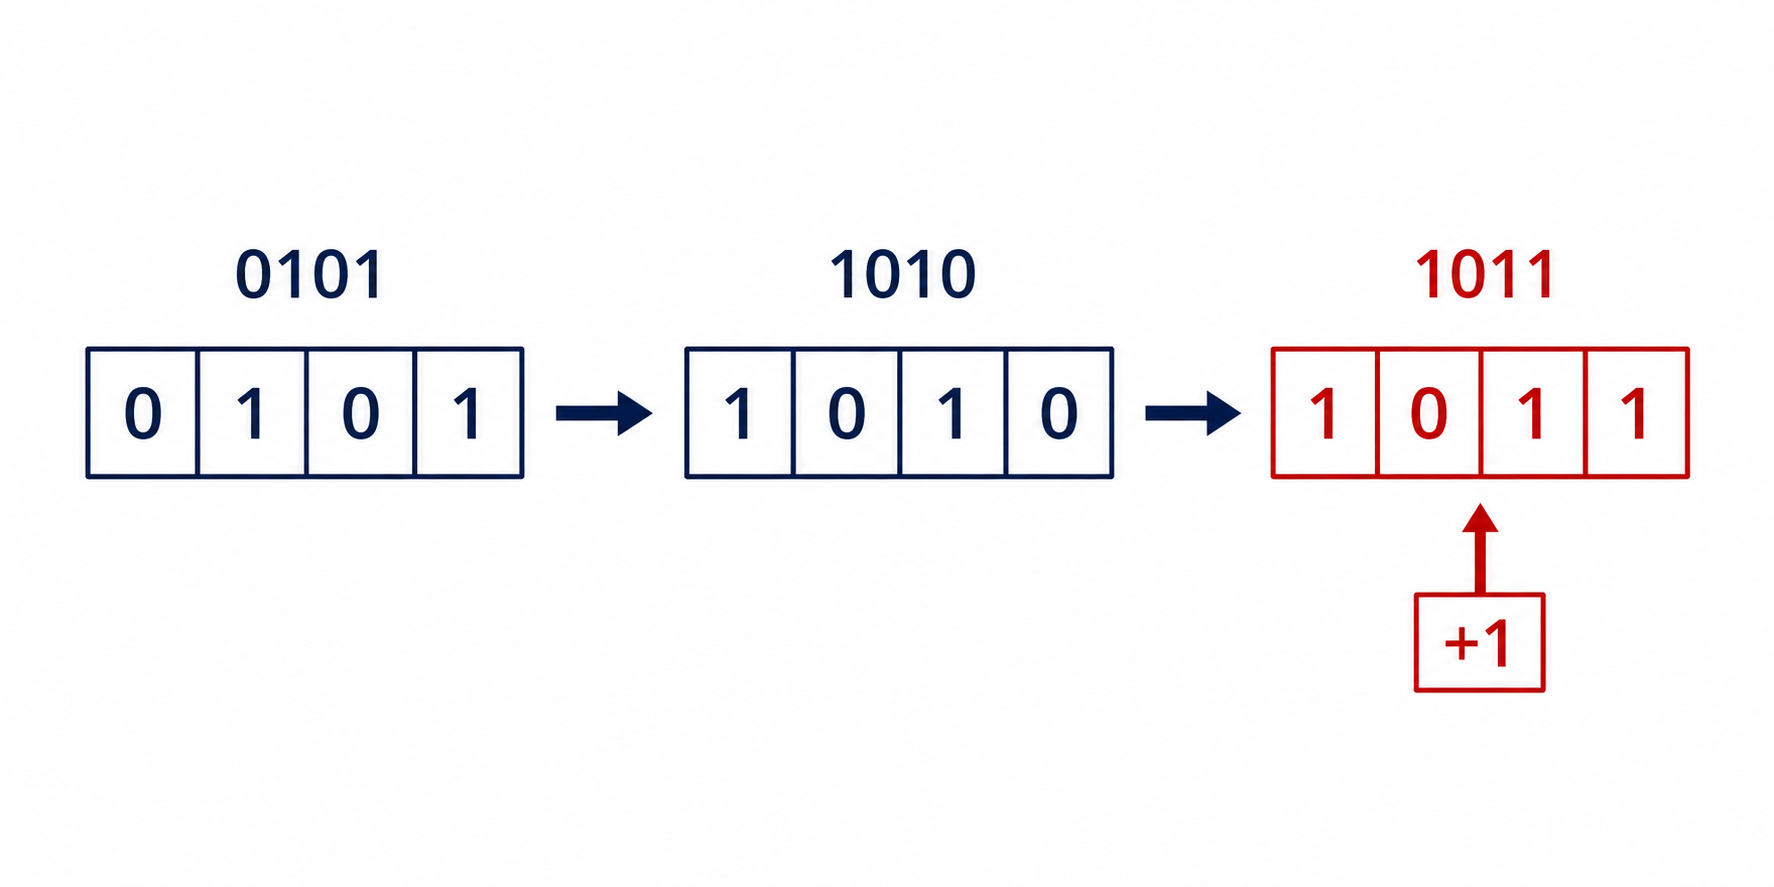
\includegraphics[width=0.62\textwidth]{Figures/png_ready/28-2s-complement-manual.png}
    \caption{แผนภาพแสดงขั้นตอนการสร้างส่วนเติมเต็มสอง}
    \label{fig:2s-complement}
\end{figure}

\label{ssec:twos-complement}
รูปที่~\ref{fig:2s-complement} แสดงลำดับการทำงานจากซ้ายไปขวา เริ่มจาก $0101$ ซึ่งเป็นจำนวนบวก กลับค่าบิตทีละตำแหน่งเป็น $1010$ แล้วบวก $0001$ ตามลูกศร ผลลัพธ์คือ $1011$ ซึ่งใช้แทนค่าลบของจำนวนเดิมในระบบส่วนเติมเต็มสองแบบ 4 บิต
วิธีที่ใช้กันมากที่สุดในคอมพิวเตอร์ปัจจุบัน

\begin{thrm}
ในระบบ 2's complement ขนาด $n$ bits:
\begin{enumerate}
    \item ค่าบวก เหมือน unsigned
    \item ค่าลบ คือ กลับ bit ทุก bit แล้วบวก 1 หรือเทียบเท่ากับ $2^n - |x|$
    \item ช่วง $-2^{n-1}$ ถึง $+(2^{n-1}-1)$
    \item มี 0 แบบเดียว คือ $00000000$
    \item การบวกปกติใช้ได้เลยโดยไม่ต้อง special case
\end{enumerate}
\label{thrm:twos-complement}
\end{thrm}

\begin{prop}
ในระบบ 2's complement $n$ bits สำหรับจำนวนเต็ม $x$ ใดๆ จะได้ว่า $-x \equiv 2^n - x \pmod{2^n}$ และ $-x$ หาได้โดยการกลับ bit ทุก bit แล้วบวก 1
\end{prop}

\begin{ex}[การหาค่า 2's Complement]
จงหาค่า $-45$ ในระบบ 2's complement ขนาด 8 บิต
\end{ex}
\begin{solution}
\begin{align*}
+45 &= (00101101)_2\\
-45 &= (11010011)_2 \quad (\text{กลับบิตแล้วบวก 1})
\end{align*}
ตรวจสอบ: $(00101101)_2 + (11010011)_2 = (1\,00000000)_2 \equiv (00000000)_2$ (ตัดบิตทดซ้ายสุดทิ้ง) \solhere
\end{solution}

\begin{ex}
หาค่าของ $11010011_2$ ในระบบ 2's complement 8 bits:
\end{ex}
\begin{solution}
บิตซ้ายสุดเป็น 1 จึงเป็นจำนวนลบ หาค่าสัมบูรณ์โดยกลับบิตแล้วบวก 1
\begin{align*}
(11010011)_2 \xrightarrow{\text{กลับบิต}} (00101100)_2 \xrightarrow{+1} (00101101)_2 = 45
\end{align*}
$\therefore (11010011)_2 = -45$
\end{solution}

\begin{thrm}
ช่วงค่าในระบบ 2's complement $n$ bits:
\begin{enumerate}
    \item ค่าบวกมากที่สุด คือ $2^{n-1} - 1$ (เช่น 127 ใน 8 bits)
    \item ค่าลบน้อยที่สุด คือ $-2^{n-1}$ (เช่น -128 ใน 8 bits)
    \item ไม่มี $-0$ เพราะ $-128$ ใช้ $10000000_2$
\end{enumerate}
\label{thrm:twos-complement-range}
\end{thrm}

\section{การบวกและลบในฐานสิบหก}
\zlabel{sec:hex-arithmetic}
การบวกและลบในฐานสิบหกมีหลักการเหมือนกับฐานสิบทุกประการ แต่ตัวเลขสูงสุดในแต่ละหลักคือ $F$ (ค่า 15) แทนที่จะเป็น $9$ การบวกจึงต้องทดเมื่อผลลัพธ์เกิน $F$ ซึ่งเทียบเท่ากับการทดเมื่อผลบวกเกิน 9 ในฐานสิบ ความเข้าใจในการดำเนินการฐานสิบหกมีความสำคัญในการเขียนโปรแกรมระดับต่ำ การแก้ไขข้อมูลในหน่วยความจำ และการใช้เครื่องมือ debug

\begin{thrm}
ถ้าผลบวกของแต่ละหลักเกิน $F_{16}$ ให้ทด 1 ไปหลักซ้าย และเขียนผลลัพธ์ลบ 16
โดยที่ $F_{16}$ มีค่าเท่ากับ 15 ในฐานสิบ การทด 1 หลักในฐานสิบหกหมายถึงการบวก $16$ เข้าไปในผลลัพธ์
\end{thrm}
\label{thrm:hex-addition-carry}

\begin{ex}
บวก $(3A5)_{16}$ กับ $(1F7)_{16}$:
\end{ex}

\begin{solution}
\[
\begin{array}{r}
3A5 \\
+\,1F7 \\
\hline
59C
\end{array}
\]
$\therefore (3A5)_{16} + (1F7)_{16} = (59C)_{16}$

ตรวจสอบ: $(3A5)_{16} = 933_{10}$, $(1F7)_{16} = 503_{10}$, และ $933+503 = 1436 = (59C)_{16}$ \checkmark
\end{solution}

\begin{ex}
ลบ $(9F2)_{16}$ ด้วย $(3A4)_{16}$:
\end{ex}

\begin{solution}
\[
\begin{array}{r}
9F2 \\
-\,3A4 \\
\hline
64E
\end{array}
\]
$\therefore (9F2)_{16} - (3A4)_{16} = (64E)_{16}$

ตรวจสอบ: $(9F2)_{16} = 2546_{10}$, $(3A4)_{16} = 932_{10}$, และ $2546-932 = 1614 = (64E)_{16}$ \checkmark
\end{solution}

\section{IEEE 754  การแทนทศนิยมในคอมพิวเตอร์}
\zlabel{sec:ieee754}
มาตรฐาน IEEE 754 (Institute of Electrical and Electronics Engineers) เป็นมาตรฐานสากลที่ใช้ในการจัดเก็บและคำนวณจำนวนจริงในรูปเลขทศนิยมลอยตัว (Floating-Point Numbers) ในหน่วยประมวลผลของคอมพิวเตอร์ทุกชนิด การเข้าใจโครงสร้าง IEEE 754 ช่วยให้โปรแกรมเมอร์เข้าใจเรื่องขอบเขตความแม่นยำและความผิดพลาดจากการปัดเศษ (Floating-point error) โดยแบ่งข้อมูลออกเป็น 3 ส่วนหลัก ได้แก่ บิตเครื่องหมาย เลขชี้กำลัง และแมนทิสซา ดังแสดงในรูปที่~\ref{fig:ieee754}

\begin{figure}[H]
    \centering
    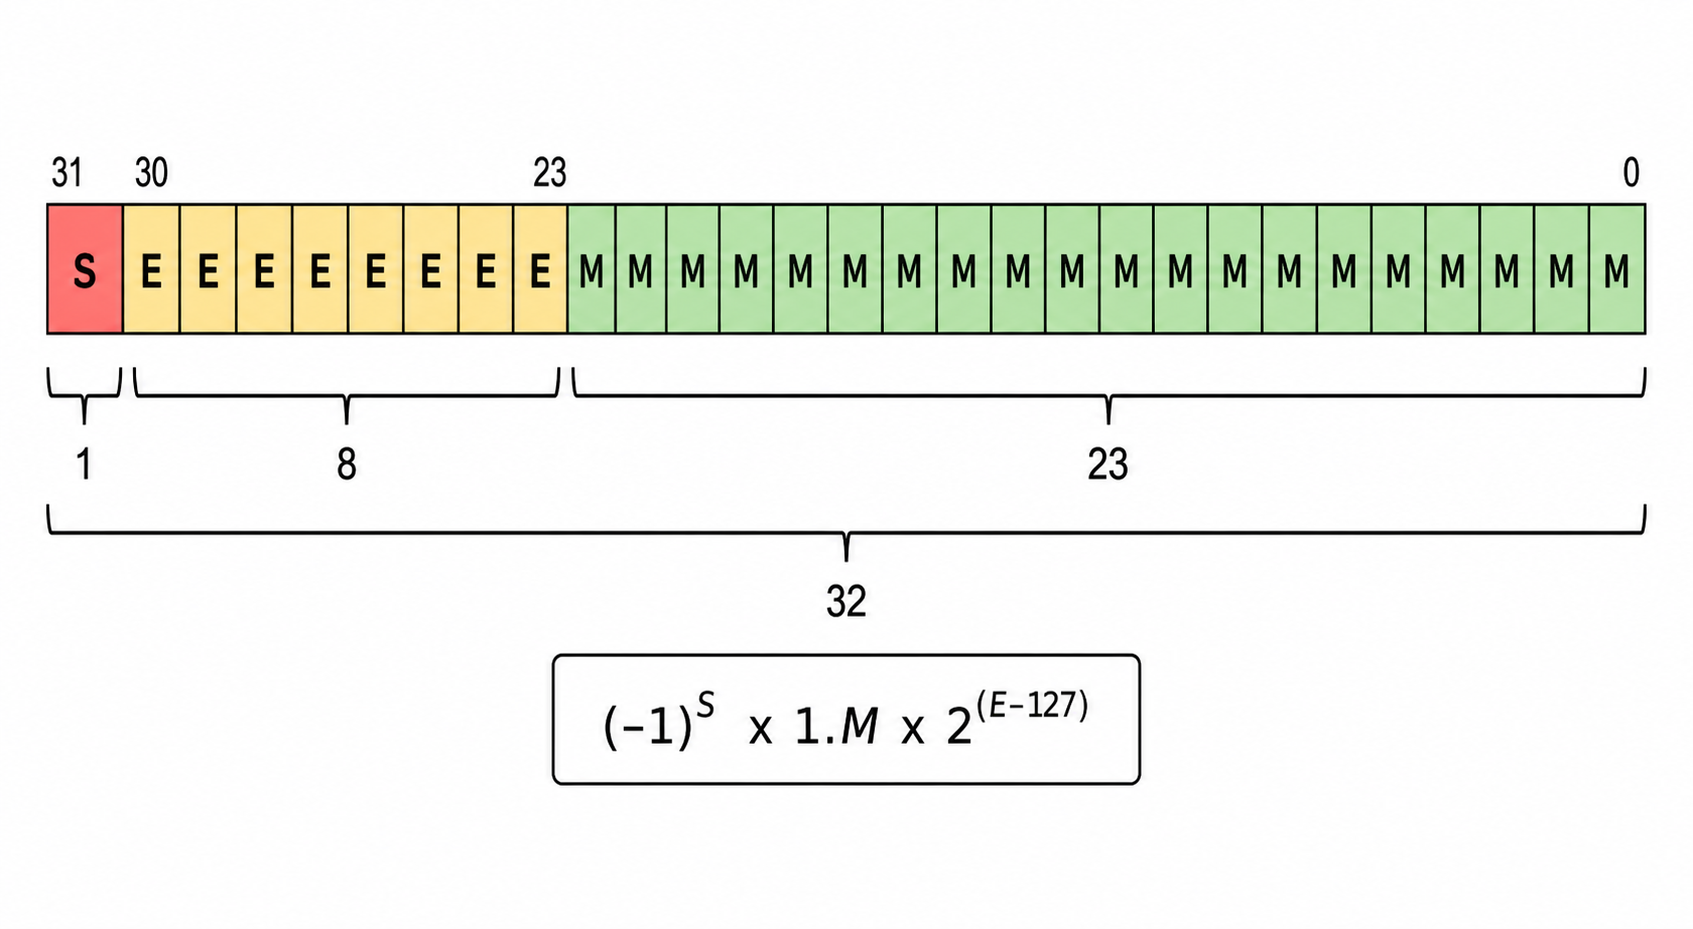
\includegraphics[width=0.62\textwidth]{Figures/png_ready/29-ieee754-manual.png}
    \caption{แผนภาพแสดงโครงสร้างการแทนเลขแบบ IEEE 754 ความละเอียดเดี่ยว}
    \label{fig:ieee754}
\end{figure}

\subsection{โครงสร้างของ IEEE 754 Single Precision (32 bits)}
\label{ssec:ieee-754-single-precision}
มาตรฐาน IEEE 754 กำหนดวิธีเก็บจำนวนจริงในรูปเลขทศนิยมลอยตัว (floating point) โดยแบ่งบิตออกเป็นส่วน ๆ ที่มีหน้าที่ต่างกัน แบบ single precision ใช้ทั้งหมด 32 บิต

\begin{definition}[โครงสร้าง IEEE 754 Single Precision]
\index{IEEE 754!โครงสร้าง}
จำนวน single precision 32 bits แบ่งเป็น 3 ส่วน ดังนี้
\begin{enumerate}
    \item บิตเครื่องหมาย ($S$) ขนาด 1 บิต (0 แทนบวก, 1 แทนลบ)
    \item เลขชี้กำลัง ($E$) ขนาด 8 บิต (ปรับเอียงด้วยไบแอส)
    \item ส่วนเศษ ($F$) ขนาด 23 บิต (แมนทิสซา)
\end{enumerate}
ค่าจริงของจำนวนคือ
\[ (-1)^S \times 1.F \times 2^{E-127} \]
\end{definition}
\label{thrm:ieee-754-structure}

โดยที่ $S$ คือ sign bit กำหนดเครื่องหมายของจำนวน, $E$ คือ biased exponent ซึ่งมี bias เท่ากับ 127 สำหรับ single precision และ $F$ คือ fraction (mantissa) ที่อยู่หลังจุดทศนิยม

\begin{prop}
เหตุผลที่ใช้ bias 127 สำหรับ single precision คือเพื่อให้ค่า exponent ที่เก็บเป็นจำนวนไม่ติดลบตั้งแต่ 0 ถึง 255 ทำให้การเปรียบเทียบทำได้ง่าย สำหรับ normalized numbers ค่า exponent field จะอยู่ในช่วง 1 ถึง 254 จึงทำให้ค่า exponent จริงอยู่ในช่วง $-126$ ถึง $+127$ ส่วนค่า exponent field 0 และ 255 สงวนไว้สำหรับ subnormal numbers, zero, infinity และ NaN
\end{prop}

\begin{ex}
จำนวน $3.14$ ในระบบ IEEE 754 single precision:
\end{ex}
\begin{solution}
\begin{align*}
3.14 &\approx (11.00100011\ldots)_2 \quad (\text{ค่าประมาณ})\\
     &= 1.100100011\ldots \times 2^{1} \quad (\text{normalize})\\
S &= 0\\
E &= 1 + 127 = 128 = (10000000)_2\\
F &= 100100011\ldots \quad (\text{23 บิต})
\end{align*}
\solhere
\end{solution}

\begin{ex}
จำนวน $-0.5$ ในระบบ IEEE 754 single precision:
\end{ex}
\begin{solution}
\begin{align*}
0.5 &= (0.1)_2\\
    &= 1.0 \times 2^{-1} \quad (\text{normalize})\\
S &= 1 \quad (\text{ลบ})\\
E &= -1 + 127 = 126 = (01111110)_2\\
F &= (0\ldots0)_2 \quad (\text{23 บิต})
\end{align*}
$\therefore -0.5 = (10111111\,00000000000000000000000)_2 = (\mathrm{BF000000})_{16} = \texttt{0xBF000000}$
\end{solution}

\begin{rem}
ค่า exponent ใน IEEE 754 ใช้ biased notation โดยบวก bias 127 เข้าไปก่อนเก็บ ทำให้ค่าที่เก็บได้เป็นจำนวนไม่ติดลบ วิธีนี้ทำให้การเปรียบเทียบ exponent ทำได้ง่ายเหมือนจำนวนไม่คิดเครื่องหมาย
\end{rem}
\label{rem:ieee-bias}

\subsection{Special Values ใน IEEE 754}
\label{ssec:ieee-754-special-values}
นอกจากการเก็บจำนวนปกติแล้ว IEEE 754 ยังสงวนรูปแบบบิตบางแบบไว้แทนค่าพิเศษ เช่น ศูนย์ อนันต์ และค่าที่ไม่ใช่จำนวน เพื่อให้การคำนวณจัดการกรณีขอบเขตได้อย่างสอดคล้องกัน

\begin{definition}[ค่าพิเศษในมาตรฐาน IEEE 754]
\index{IEEE 754!ค่าพิเศษ}
มาตรฐาน IEEE 754 กำหนดค่าพิเศษไว้ดังนี้
\begin{enumerate}
    \item ศูนย์ (Zero) เมื่อเลขชี้กำลัง $E = 0$ และส่วนเศษ $F = 0$
    \item จำนวนแบบบิตต่ำกว่าปกติ (Denormalized) เมื่อเลขชี้กำลัง $E = 0$ และส่วนเศษ $F \neq 0$
    \item อนันต์ (Infinity) เมื่อเลขชี้กำลัง $E = 255$ และส่วนเศษ $F = 0$
    \item ไม่ใช่จำนวน (NaN) เมื่อเลขชี้กำลัง $E = 255$ และส่วนเศษ $F \neq 0$
\end{enumerate}
\end{definition}
\label{thrm:ieee-special-values}

\begin{ex}[การแทนค่าพิเศษในระบบ IEEE 754 แบบ Single Precision]
จงแสดงการแทนบิตแบบ IEEE 754 Single Precision (32 บิต) สำหรับค่าพิเศษ ได้แก่ $+0$, $-0$, $+\infty$ และ $-\infty$ พร้อมอธิบายองค์ประกอบของ Sign ($S$), Exponent ($E$) และ Fraction ($F$) ในแต่ละกรณี
\end{ex}
\begin{solution}
ในมาตรฐาน IEEE 754 Single Precision (32 บิต) ประกอบด้วย Sign ($S$, 1 บิต), Exponent ($E$, 8 บิต) และ Fraction ($F$, 23 บิต) โดยค่าพิเศษแต่ละค่ามีโครงสร้างบิตและการอธิบายดังนี้:

\begin{itemize}[leftmargin=1.5em,itemsep=0.5em]
    \item \textbf{ค่า $+0$:} เครื่องหมายเป็นบวก ($S=0$), Exponent เป็น 0 ทั้งหมด ($E=00000000_2$) และส่วนเศษเป็น 0 ทั้งหมด ($F=0_2$)
    \[ +0 = \underbrace{0}_{S} \ \underbrace{00000000}_{E} \ \underbrace{00000000000000000000000}_{F} \]
    
    \item \textbf{ค่า $-0$:} เครื่องหมายเป็นลบ ($S=1$), Exponent เป็น 0 ทั้งหมด ($E=00000000_2$) และส่วนเศษเป็น 0 ทั้งหมด ($F=0_2$)
    \[ -0 = \underbrace{1}_{S} \ \underbrace{00000000}_{E} \ \underbrace{00000000000000000000000}_{F} \]
    
    \item \textbf{ค่า $+\infty$ (Positive Infinity):} เครื่องหมายเป็นบวก ($S=0$), Exponent เป็น 1 ทั้งหมด ($E=11111111_2 = 255$) และส่วนเศษเป็น 0 ทั้งหมด ($F=0_2$)
    \[ +\infty = \underbrace{0}_{S} \ \underbrace{11111111}_{E} \ \underbrace{00000000000000000000000}_{F} \]
    
    \item \textbf{ค่า $-\infty$ (Negative Infinity):} เครื่องหมายเป็นลบ ($S=1$), Exponent เป็น 1 ทั้งหมด ($E=11111111_2 = 255$) และส่วนเศษเป็น 0 ทั้งหมด ($F=0_2$)
    \[ -\infty = \underbrace{1}_{S} \ \underbrace{11111111}_{E} \ \underbrace{00000000000000000000000}_{F} \]
\end{itemize}
\solhere
\end{solution}

\begin{rem}
\textbf{Machine Epsilon} คือค่าที่เล็กที่สุดที่บวกกับ 1 แล้วได้ค่าต่างจาก 1 ใน floating-point สำหรับ single precision คือ $2^{-23} \approx 1.19 \times 10^{-7}$ นี่คือขอบเขตของความแม่นยำในการคำนวณทศนิยม
\end{rem}
\label{rem:machine-epsilon}

\section{การแทนข้อมูลในคอมพิวเตอร์}
\zlabel{sec:data-representation}
คอมพิวเตอร์แทนทุกสิ่งด้วย bits ข้อมูลประเภทต่างๆ เช่น ตัวอักษร รูปภาพ เสียง ล้วนแปลงเป็นตัวเลขก่อนประมวลผล การเข้าใจวิธีการแทนข้อมูลจึงเป็นพื้นฐานสำคัญสำหรับการเขียนโปรแกรมและการทำงานของระบบคอมพิวเตอร์ทุกระดับ~\cite{patterson2020organization}
\label{sec:data-representation}

\subsection{ASCII (American Standard Code for Information Interchange)}
ASCII ใช้ 7 bits (หรือ 8 bits รวม parity) แทนอักขระ 128 ตัว

\begin{thrm}
ASCII แบ่งช่วงรหัสได้ดังนี้

\begin{enumerate}
    \item 0--31 คือ ตัวควบคุม (control characters)
    \item 32--47 คือ ช่องว่างและเครื่องหมายพิเศษ (!, ", \#, ...)
    \item 48--57 คือ ตัวเลข 0--9
    \item 65--90 คือ ตัวอักษรภาษาอังกฤษพิมพ์ใหญ่ A--Z
    \item 97--122 คือ ตัวอักษรภาษาอังกฤษพิมพ์เล็ก a--z
\end{enumerate}
\end{thrm}
\label{thrm:ascii-ranges}

\begin{table}[H]
\centering
\caption{ตาราง ASCII Code บางส่วน}
\label{tab:ascii}
\begin{tabular}{|c|c|c|}
\hline
อักขระ & ASCII (decimal) & ASCII (hex) \\
\hline
'A' & 65 & 41 \\
'B' & 66 & 42 \\
'0' & 48 & 30 \\
'/' & 47 & 2F \\
'a' & 97 & 61 \\
'\{' & 123 & 7B \\
\hline
\end{tabular}
\end{table}

\begin{ex}
คำ ``Hi'' ใน ASCII hexadecimal:
\end{ex}
\begin{solution}
\begin{align*}
\text{`H'} &= \texttt{0x48}\\
\text{`i'} &= \texttt{0x69}
\end{align*}
$\therefore$ ``Hi'' $= \texttt{0x4869}$ \solhere
\end{solution}

\begin{rem}
ASCII มีข้อจำกัดในการแทนอักขระภาษาอื่น เช่น ภาษาไทย จีน ญี่ปุ่น จึงพัฒนา Unicode ขึ้นมาเพื่อแก้ปัญหานี้
\end{rem}
\label{rem:ascii-limitation}

\subsection{Unicode}
ระบบรหัสยูนิโคด (Unicode) ถูกพัฒนาขึ้นเพื่อแก้ข้อจำกัดของรหัส ASCII และตารางรหัสท้องถิ่นที่สามารถแทนอักขระได้เพียงจำนวนจำกัด โดยกำหนดจุดรหัส (Code Point) ที่เป็นเอกลักษณ์เฉพาะให้แก่อักขระ สัญลักษณ์ และตัวอักษรทุกภาษาทั่วโลก การเข้าใจรูปแบบการเข้ารหัสของยูนิโคดช่วยให้โปรแกรมเมอร์จัดการข้อมูลข้อความหลายภาษาได้อย่างถูกต้องโดยไม่เกิดปัญหาอักขระต่างดาว (Moibake)

\begin{definition}[การเข้ารหัสยูนิโคด]
\index{ยูนิโคด!การเข้ารหัส}
ระบบยูนิโคดมีรูปแบบการเข้ารหัสหลักดังนี้
\begin{enumerate}
    \item UTF-8 ใช้ขนาด 1 ถึง 4 ไบต์ นิยมใช้แพร่หลายที่สุดบนอินเทอร์เน็ต
    \item UTF-16 ใช้ขนาด 2 ถึง 4 ไบต์ นิยมใช้ในระบบปฏิบัติการ Windows และภาษา Java
    \item UTF-32 ใช้ขนาด 4 ไบต์คงที่ต่อหนึ่งอักขระ
\end{enumerate}
\end{definition}
\label{thrm:unicode-encodings}

\begin{ex}[การเข้ารหัสอักขระไทยในระบบ UTF-8]
จงแสดงการเข้ารหัสอักขระไทย `ก' (U+0E01) และ `ข' (U+0E02) ในระบบ UTF-8 แบบ 3 ไบต์
\end{ex}
\begin{solution}
\begin{align*}
\text{`ก' (U+0E01)} &= \texttt{0xE0 0xB8 0x81} \quad (\text{3 ไบต์})\\
\text{`ข' (U+0E02)} &= \texttt{0xE0 0xB8 0x82} \quad (\text{3 ไบต์})
\end{align*}
$\therefore$ ``กข'' $= \texttt{0xE0B881E0B882}$ \solhere
\end{solution}

\sectionbanner{สรุปบทเรียน}
\zlabel{sec:chapter-summary}
บทนี้เริ่มจากระบบเลขฐานสิบที่มนุษย์ใช้ในชีวิตประจำวัน แล้วเข้าสู่ระบบเลขฐานสองซึ่งเป็นภาษาของคอมพิวเตอร์ ฐานแปดและฐานสิบหกช่วยให้เขียนเลขฐานสองได้กระชับและแปลงกลับไปมากับฐานสองได้สะดวก การแปลงระหว่างฐานอาศัยการหารต่อเนื่องสำหรับส่วนจำนวนเต็มและการคูณต่อเนื่องสำหรับส่วนทศนิยม ถัดจากนั้นเป็นการบวก ลบ คูณ และหารในฐานสองและฐานสิบหก การแทนจำนวนเต็มลบด้วยวิธี signed magnitude, 1's complement และ 2's complement และการแทนจำนวนจริงตามมาตรฐาน IEEE 754 ก่อนปิดท้ายด้วยการแทนอักขระด้วยรหัส ASCII และ Unicode

ความเข้าใจในระบบเลขฐานเป็นพื้นฐานสำหรับการศึกษาสถาปัตยกรรมคอมพิวเตอร์ การเขียนโปรแกรมระดับต่ำ และการเข้ารหัสข้อมูล~\cite{rosen2019discrete}

\clearpage
\sectionbanner{แบบฝึกหัดท้ายบท}
\zlabel{sec:exercises}
\exercisepart{ส่วนที่ 1: การแปลงฐาน}
\begin{exercise}
แปลงต่อไปนี้เป็นฐานสิบ
\begin{enumerate}
    \item $(1011)_2$
    \item $(10010)_2$
    \item $(72)_8$
    \item $(5F)_{16}$
    \item $(1001.101)_2$
    \item $(3A.8)_{16}$
\end{enumerate}
\end{exercise}

\begin{exercise}
แปลงต่อไปนี้เป็นฐานสอง
\begin{enumerate}
    \item $45_{10}$
    \item $127_{10}$
    \item $0.625_{10}$
    \item $0.8125_{10}$
    \item $73_{10}$
    \item $255_{10}$
\end{enumerate}
\end{exercise}

\begin{exercise}
แปลงต่อไปนี้เป็นฐานแปดและฐานสิบหก
\begin{enumerate}
    \item $(11010110)_2$
    \item $(10101010)_2$
\end{enumerate}
\end{exercise}

\begin{exercise}
แปลงต่อไปนี้เป็นฐานสิบ
\begin{enumerate}
    \item $(A1B)_{16}$
    \item $(777)_8$
    \item $(3CD.2A)_{16}$
\end{enumerate}
\end{exercise}

\exercisepart{ส่วนที่ 2: การดำเนินการฐานสอง}
\begin{exercise}
จงหา
\begin{enumerate}
    \item $(1011)_2 + (1101)_2$
    \item $(10001)_2 - (111)_2$
    \item $(1101)_2 \times (101)_2$
    \item $(11000)_2 \div (100)_2$
\end{enumerate}
\end{exercise}

\begin{exercise}
จงหา 2's complement ของ $(45)_{10}$ ใน 8 bits
\end{exercise}

\begin{exercise}
กำหนดให้ในระบบ 2's complement ขนาด 8 bits จงหาค่าฐานสิบของจำนวนต่อไปนี้
\begin{enumerate}
    \item $01101001_2$
    \item $10110110_2$
\end{enumerate}
\end{exercise}

\exercisepart{ส่วนที่ 3: การดำเนินการฐานสิบหก}
\begin{exercise}
จงหา
\begin{enumerate}
    \item $(3A7)_{16} + (1B9)_{16}$
    \item $(FF)_{16} - (A1)_{16}$
    \item $(2F)_{16} \times (4)_{16}$
\end{enumerate}
\end{exercise}

\exercisepart{ส่วนที่ 4: การแทนข้อมูลและ IEEE 754}
\begin{exercise}
เขียนคำต่อไปนี้ในรูป hexadecimal (ASCII)
\begin{enumerate}
    \item ``Hi''
    \item ``OK''
\end{enumerate}
\end{exercise}

\begin{exercise}
อธิบายข้อดีข้อเสียของ signed magnitude, 1's complement และ 2's complement
\end{exercise}

\begin{exercise}
จำนวน $1.0$ ใน IEEE 754 single precision มีค่า hex คือ $3F800000$ จงอธิบายว่าแต่ละ field คืออะไร
\end{exercise}

\answerkeyhead
\exercisepart{เฉลยส่วนที่ 1: การแปลงฐาน}
\begin{enumerate}[label={},leftmargin=0pt,itemsep=0.6em]
    \item
    \begin{enumerate}[label=\textbf{\thechapter.\arabic{enumi}.\arabic*}]
        \item $1011_2 = 1 \times 8 + 1 \times 2 + 1 \times 1 = 11$
        \item $10010_2 = 1 \times 16 + 1 \times 2 = 18$
        \item $72_8 = 7 \times 8 + 2 = 58$
        \item $5F_{16} = 5 \times 16 + 15 = 95$
        \item $1001.101_2 = 9 + 0.5 + 0.125 = 9.625$
        \item $3A.8_{16} = 3 \times 16 + 10 + 8/16 = 58.5$
    \end{enumerate}

    \item
    \begin{enumerate}[label=\textbf{\thechapter.\arabic{enumi}.\arabic*}]
        \item $45_{10} = 101101_2$
        \item $127_{10} = 1111111_2$
        \item $0.625_{10} = 0.101_2$
        \item $0.8125_{10} = 0.1101_2$
        \item $73_{10} = 1001001_2$
        \item $255_{10} = 11111111_2$
    \end{enumerate}

    \item
    \begin{enumerate}[label=\textbf{\thechapter.\arabic{enumi}.\arabic*}]
        \item $(11010110)_2 \to$ ฐานแปด: $(011\ 010\ 110)_2 = 326_8$; ฐานสิบหก: $(1101\ 0110)_2 = \text{D}6_{16}$
        \item $(10101010)_2 \to$ ฐานแปด: $(010\ 101\ 010)_2 = 252_8$; ฐานสิบหก: $(1010\ 1010)_2 = \text{AA}_{16}$
    \end{enumerate}

    \item
    \begin{enumerate}[label=\textbf{\thechapter.\arabic{enumi}.\arabic*}]
        \item $(A1B)_{16} = 10 \times 256 + 1 \times 16 + 11 = 2587_{10}$
        \item $(777)_8 = 7 \times 64 + 7 \times 8 + 7 = 511_{10}$
        \item $(3CD.2A)_{16} = 768 + 192 + 13 + 0.125 + 0.0390625 = 973.1640625_{10}$
    \end{enumerate}
\end{enumerate}

\exercisepart{เฉลยส่วนที่ 2: การดำเนินการฐานสอง}
\begin{enumerate}[label={},leftmargin=0pt,itemsep=0.6em]
    \setcounter{enumi}{4}
    \item
    \begin{enumerate}[label=\textbf{\thechapter.\arabic{enumi}.\arabic*}]
        \item $(1011)_2 + (1101)_2 = (11000)_2$ ($11+13=24$)
        \item $(10001)_2 - (111)_2 = (1010)_2$ ($17-7=10$)
        \item $(1101)_2 \times (101)_2 = (1000001)_2$ ($13 \times 5=65$)
        \item $(11000)_2 \div (100)_2 = (110)_2$ ($24 \div 4=6$)
    \end{enumerate}

    \item
    \begin{enumerate}[label=\textbf{\thechapter.\arabic{enumi}.\arabic*}]
        \item $45_{10} = 00101101_2 \to$ 1's complement: $11010010_2 \to$ 2's complement: $11010011_2$ (แทน $-45_{10}$)
    \end{enumerate}

    \item
    \begin{enumerate}[label=\textbf{\thechapter.\arabic{enumi}.\arabic*}]
        \item $01101001_2 \to$ บิตเครื่องหมายเป็น 0 (บวก) $= 64 + 32 + 8 + 1 = +105_{10}$
        \item $10110110_2 \to$ บิตเครื่องหมายเป็น 1 (ลบ) $\to$ กลับบิตและ $+1 \implies 01001010_2 = 74 \implies -74_{10}$
    \end{enumerate}
\end{enumerate}

\exercisepart{เฉลยส่วนที่ 3: การดำเนินการฐานสิบหก}
\begin{enumerate}[label={},leftmargin=0pt,itemsep=0.6em]
    \setcounter{enumi}{7}
    \item
    \begin{enumerate}[label=\textbf{\thechapter.\arabic{enumi}.\arabic*}]
        \item $(3A7)_{16} + (1B9)_{16} = (560)_{16}$
        \item $(FF)_{16} - (A1)_{16} = (5E)_{16}$
        \item $(2F)_{16} \times (4)_{16} = (BC)_{16}$
    \end{enumerate}
\end{enumerate}

\exercisepart{เฉลยส่วนที่ 4: การแทนข้อมูลและ IEEE 754}
\begin{enumerate}[label={},leftmargin=0pt,itemsep=0.6em]
    \setcounter{enumi}{8}
    \item
    \begin{enumerate}[label=\textbf{\thechapter.\arabic{enumi}.\arabic*}]
        \item ``Hi'' $\to$ 'H'=0x48, 'i'=0x69 $\implies \texttt{48 69}_{16}$
        \item ``OK'' $\to$ 'O'=0x4F, 'K'=0x4B $\implies \texttt{4F 4B}_{16}$
    \end{enumerate}

    \item
    \begin{enumerate}[label=\textbf{\thechapter.\arabic{enumi}.\arabic*}]
        \item Signed magnitude และ 1's complement มีศูนย์สองแบบ (+0/-0) และต้องมีวงจรลบแยกเฉพาะ; 2's complement มีศูนย์แบบเดียว ($00\dots 0$) และใช้วงจรบวกวงจรเดียวทำได้ทั้งการบวกและการลบ จึงเป็นมาตรฐานในฮาร์ดแวร์ปัจจุบัน
    \end{enumerate}

    \item
    \begin{enumerate}[label=\textbf{\thechapter.\arabic{enumi}.\arabic*}]
        \item $3F800000_{16} = \underbrace{0}_{\text{Sign (บวก)}}\ \underbrace{01111111}_{\text{Exponent } 127 \to E=0}\ \underbrace{00000000000000000000000}_{\text{Mantissa } 1.0} \implies (-1)^0 \times 1.0 \times 2^0 = 1.0$
    \end{enumerate}
\end{enumerate}

\QAChapter
\begin{enumerate}
    \item จงแปลงจำนวนต่อไปนี้เป็นเลขฐานสิบ (ก) $(10110101)_2$ (ข) $(3\mathrm{AF})_{16}$ (ค) $(257)_8$
    \item จงแปลงเลขฐานสิบต่อไปนี้เป็นฐานที่กำหนด (ก) $255$ เป็นฐานสอง (ข) $1000$ เป็นฐานสิบหก (ค) $100$ เป็นฐานแปด
    \item จงคำนวณการบวกในระบบเลขฐานสอง $(10110101)_2 + (01101011)_2$
    \item จงแทนเลข $-45$ ในรูปแบบ 2's complement แบบ 8 บิต แล้วตรวจสอบโดยบวกกับ $+45$
    \item จงอธิบายความแตกต่างระหว่าง 1's complement และ 2's complement ในการแทนจำนวนลบ
    \item จงแปลงจำนวน $(12.625)_{10}$ เป็น IEEE 754 single precision (32-bit) แสดงขั้นตอนทีละขั้น
    \item ASCII code ของตัวอักษร A คือ 65 จงหา ASCII code ของ \texttt{Hello} (5 ตัวอักษร) และอธิบายความแตกต่างระหว่าง ASCII กับ Unicode
    \item จงอธิบายว่าทำไมคอมพิวเตอร์จึงใช้ระบบเลขฐานสอง และอธิบายความสัมพันธ์ระหว่างฐานสอง ฐานแปด และฐานสิบหก
\end{enumerate}

\newpage
\sheetChapter{ระบบเลขฐาน (Number Bases)}
\section*{วัตถุประสงค์}
\begin{enumerate}
    \item เพื่อให้ผู้เรียนแปลงเลขระหว่างฐานต่างๆ ได้อย่างถูกต้อง
    \item เพื่อให้ผู้เรียนดำเนินการทางคณิตศาสตร์ในระบบเลขฐานสองได้
    \item เพื่อให้ผู้เรียนอธิบายการแทนจำนวนลบด้วย 2's complement ได้
    \item เพื่อให้ผู้เรียนอธิบายมาตรฐาน IEEE 754 และการเข้ารหัสข้อมูล ASCII/Unicode ได้
\end{enumerate}
\section*{คำชี้แจง} ให้ผู้เรียนศึกษาเนื้อหาบทระบบเลขฐาน แล้วตอบคำถามต่อไปนี้
\begin{enumerate}
    \item จงแปลง $(10011010)_2$ เป็นเลขฐานสิบ ฐานแปด และฐานสิบหก แสดงขั้นตอนการคำนวณ
    \Pointilles{3}
    \item จงแปลง $(175)_{10}$ เป็นเลขฐานสอง ฐานแปด และฐานสิบหก
    \Pointilles{3}
    \item จงบวกเลขฐานสอง $(10101010)_2 + (01010101)_2$ แสดงขั้นตอนทีละบิต
    \Pointilles{3}
    \item จงแทน $-100$ ในรูปแบบ 2's complement แบบ 8 บิต และตรวจสอบความถูกต้อง
    \Pointilles{3}
    \item จงอธิบายขั้นตอนการแปลง $(12.625)_{10}$ เป็น IEEE 754 single precision
    \Pointilles{3}
    \item จงอธิบายความแตกต่างระหว่าง ASCII และ Unicode พร้อมอธิบายว่าทำไมระบบสมัยใหม่จึงใช้ Unicode
    \Pointilles{3}
\end{enumerate}
